\section{Results}

\subsection{Communication}

 It was stated before that the requirements for our system was to get to at least 600Hz and to reach 1000Hz if possible. As shown in Table \ref{tab:UDPMeasurements}, the connexion can go up to almost 1000Hz using UDP which fulfills the requirements. Nevertheless, the jitter should not be neglected as the frequency get closer to 1000Hz the jitter will be high compared to the period and may cause unexpected behaviour in real time operation. This issue will be further discussed in the next section. However, the data show a periodic disturbance in the system originating from the computer\todo{need some kind of graphical representation of that} which increases the jitter and delay. %Addictional safety precautions should be taken to prevent those behaviour.


\begin{table}[!t]
%\centering
  $\begin{tabular}{|c|c|c|c|c|c|}
    \hline
    \text{Delay} & \text{Frequency (Hz)} & \text{RTT* delay (ms)} & \text{Jitter} & \text{Error rate (\%)}\\
    \hline
    10ms & 86 & 1.1 & 4.9E-8 & 0 \\
    \hline
    2ms & 447 & 2.1 & 3.5 & 1.2E-4 \\
    \hline
    0ms & 981 & 1.3 & 6.1E-8 & 5.1E-5 \\
    \hline
  \end{tabular}$
  *Round Time Trip\\
  **The number of data set needs to be increased for the final version
  \caption{UDP**}
  \label{tab:UDPMeasurements}
\end{table}


\begin{figure}
  \centering
  \begin{subfigure}{.45\linewidth}
    \centering
    \vspace{24pt}
    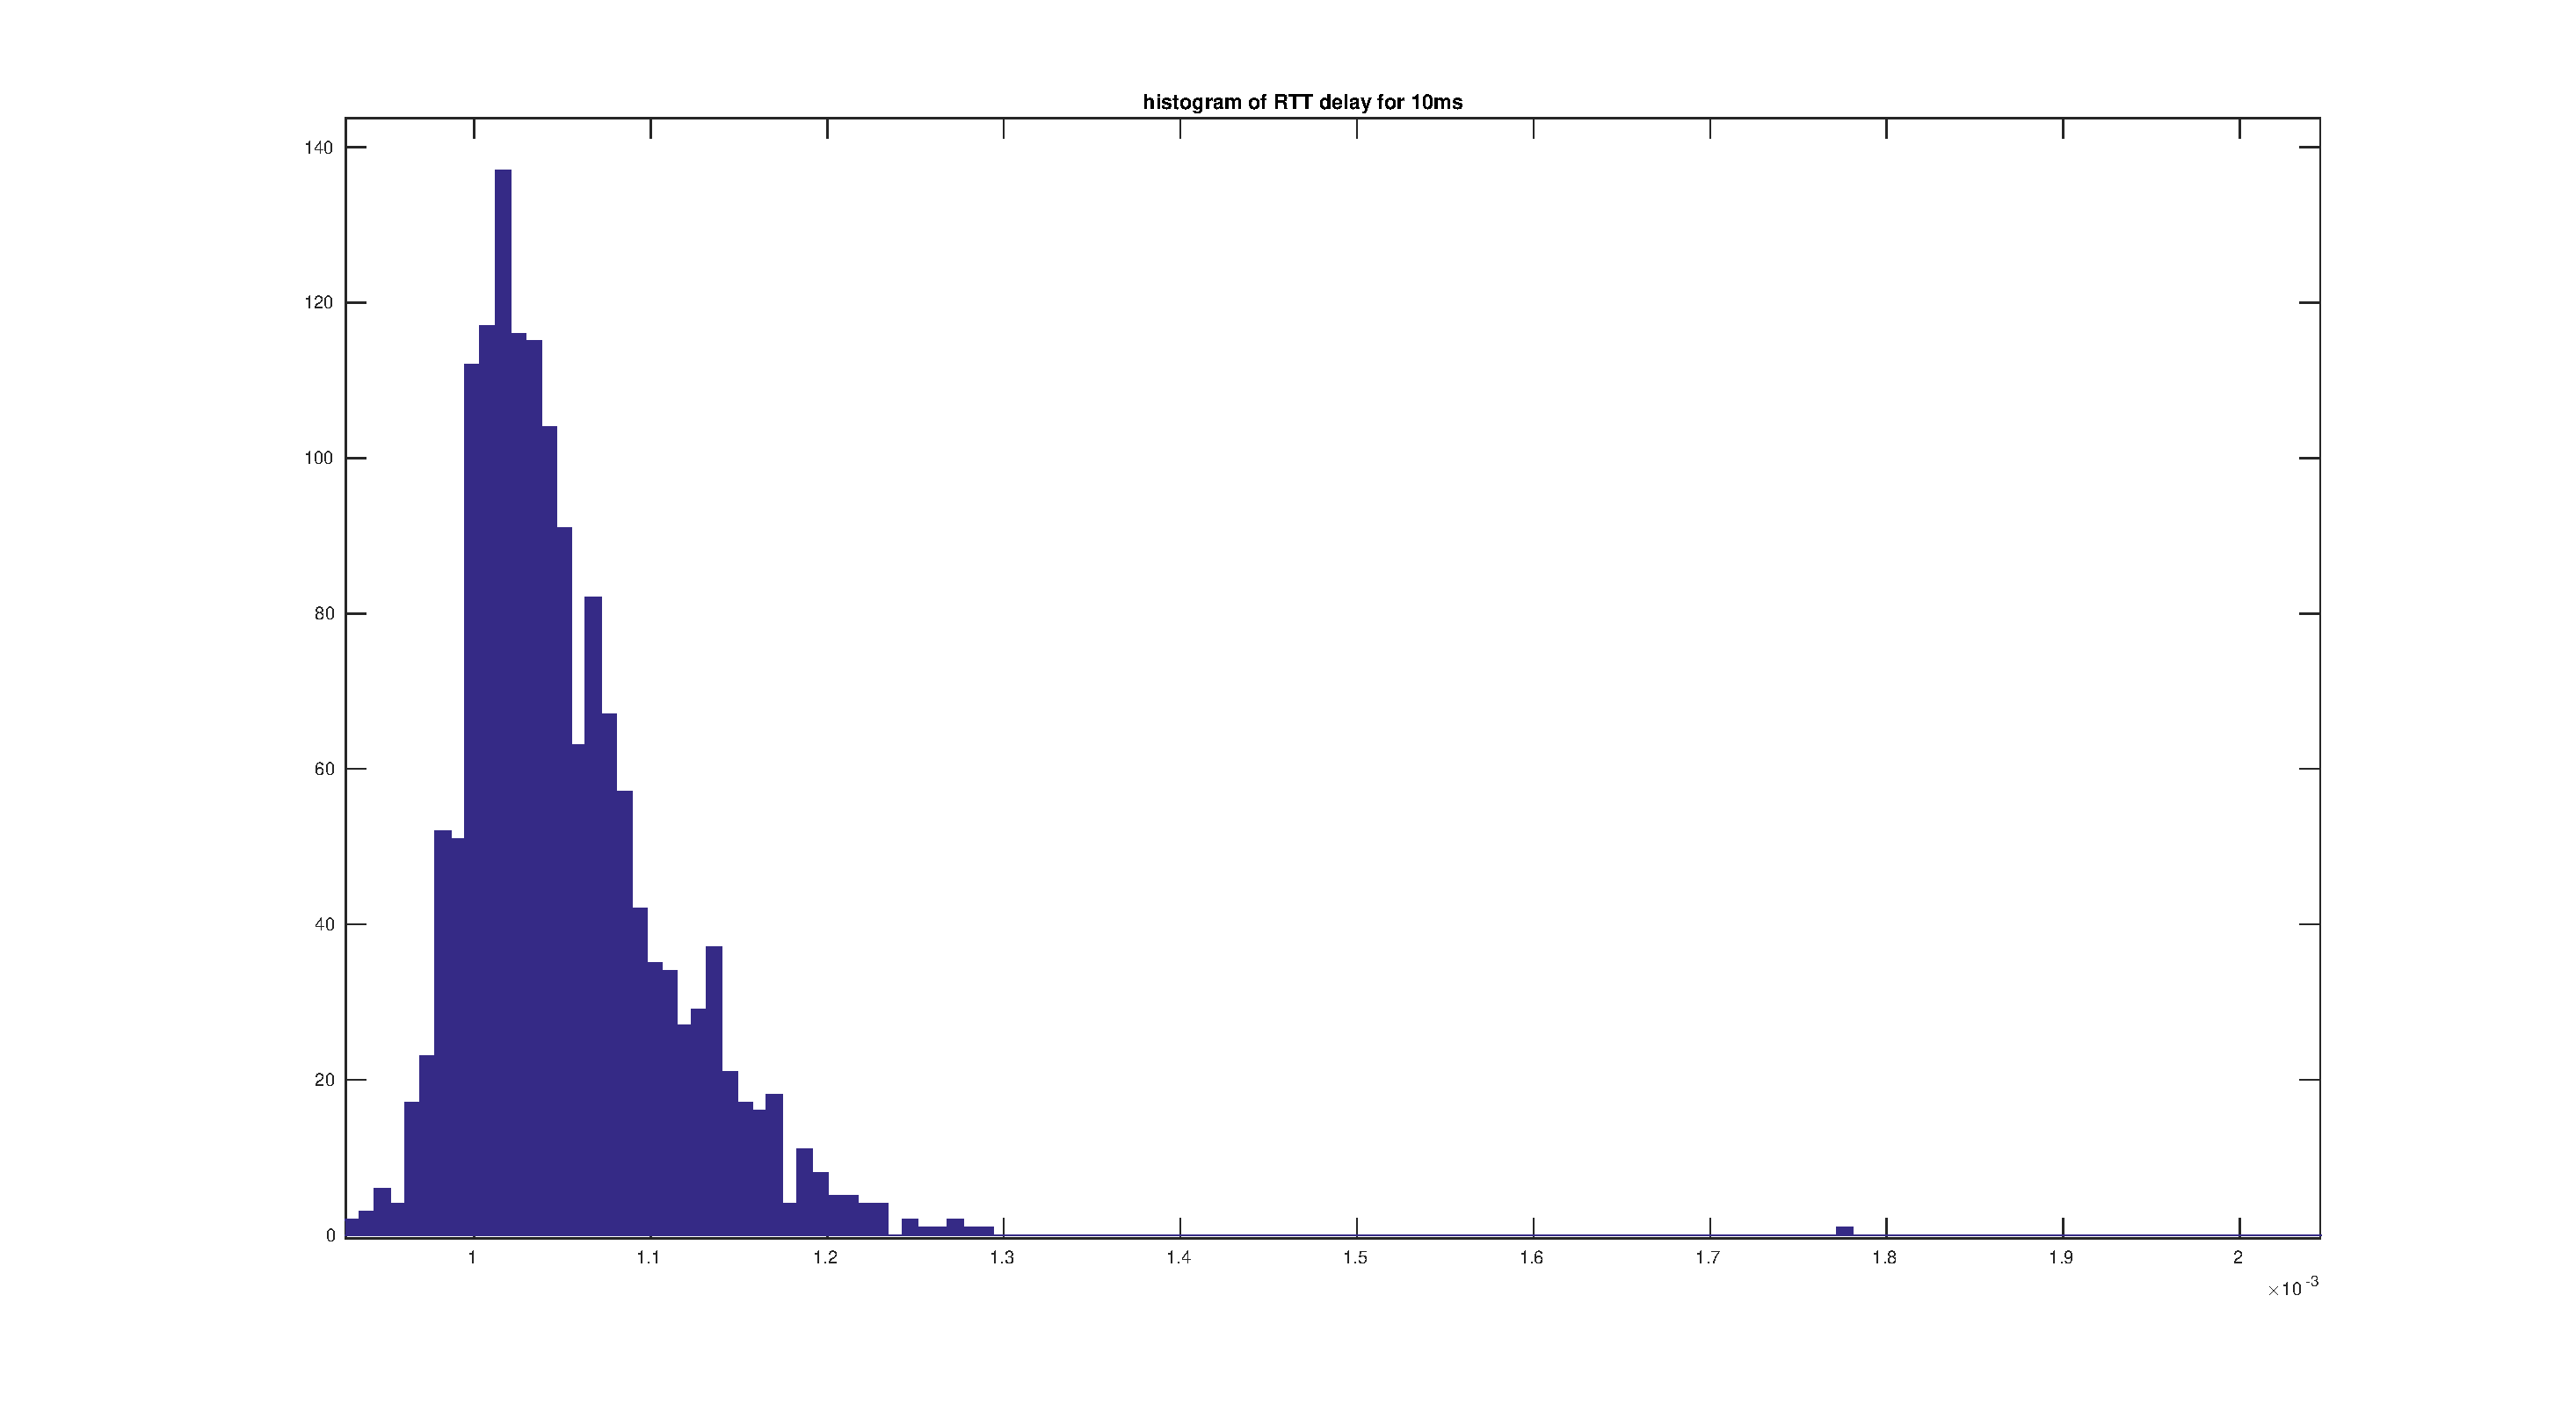
\includegraphics[width=\linewidth]{10ms}
    \caption{10ms}
    \label{fig:10ms}
  \end{subfigure}
  \begin{subfigure}{.45\linewidth}
    \centering
    \vspace{24pt}
    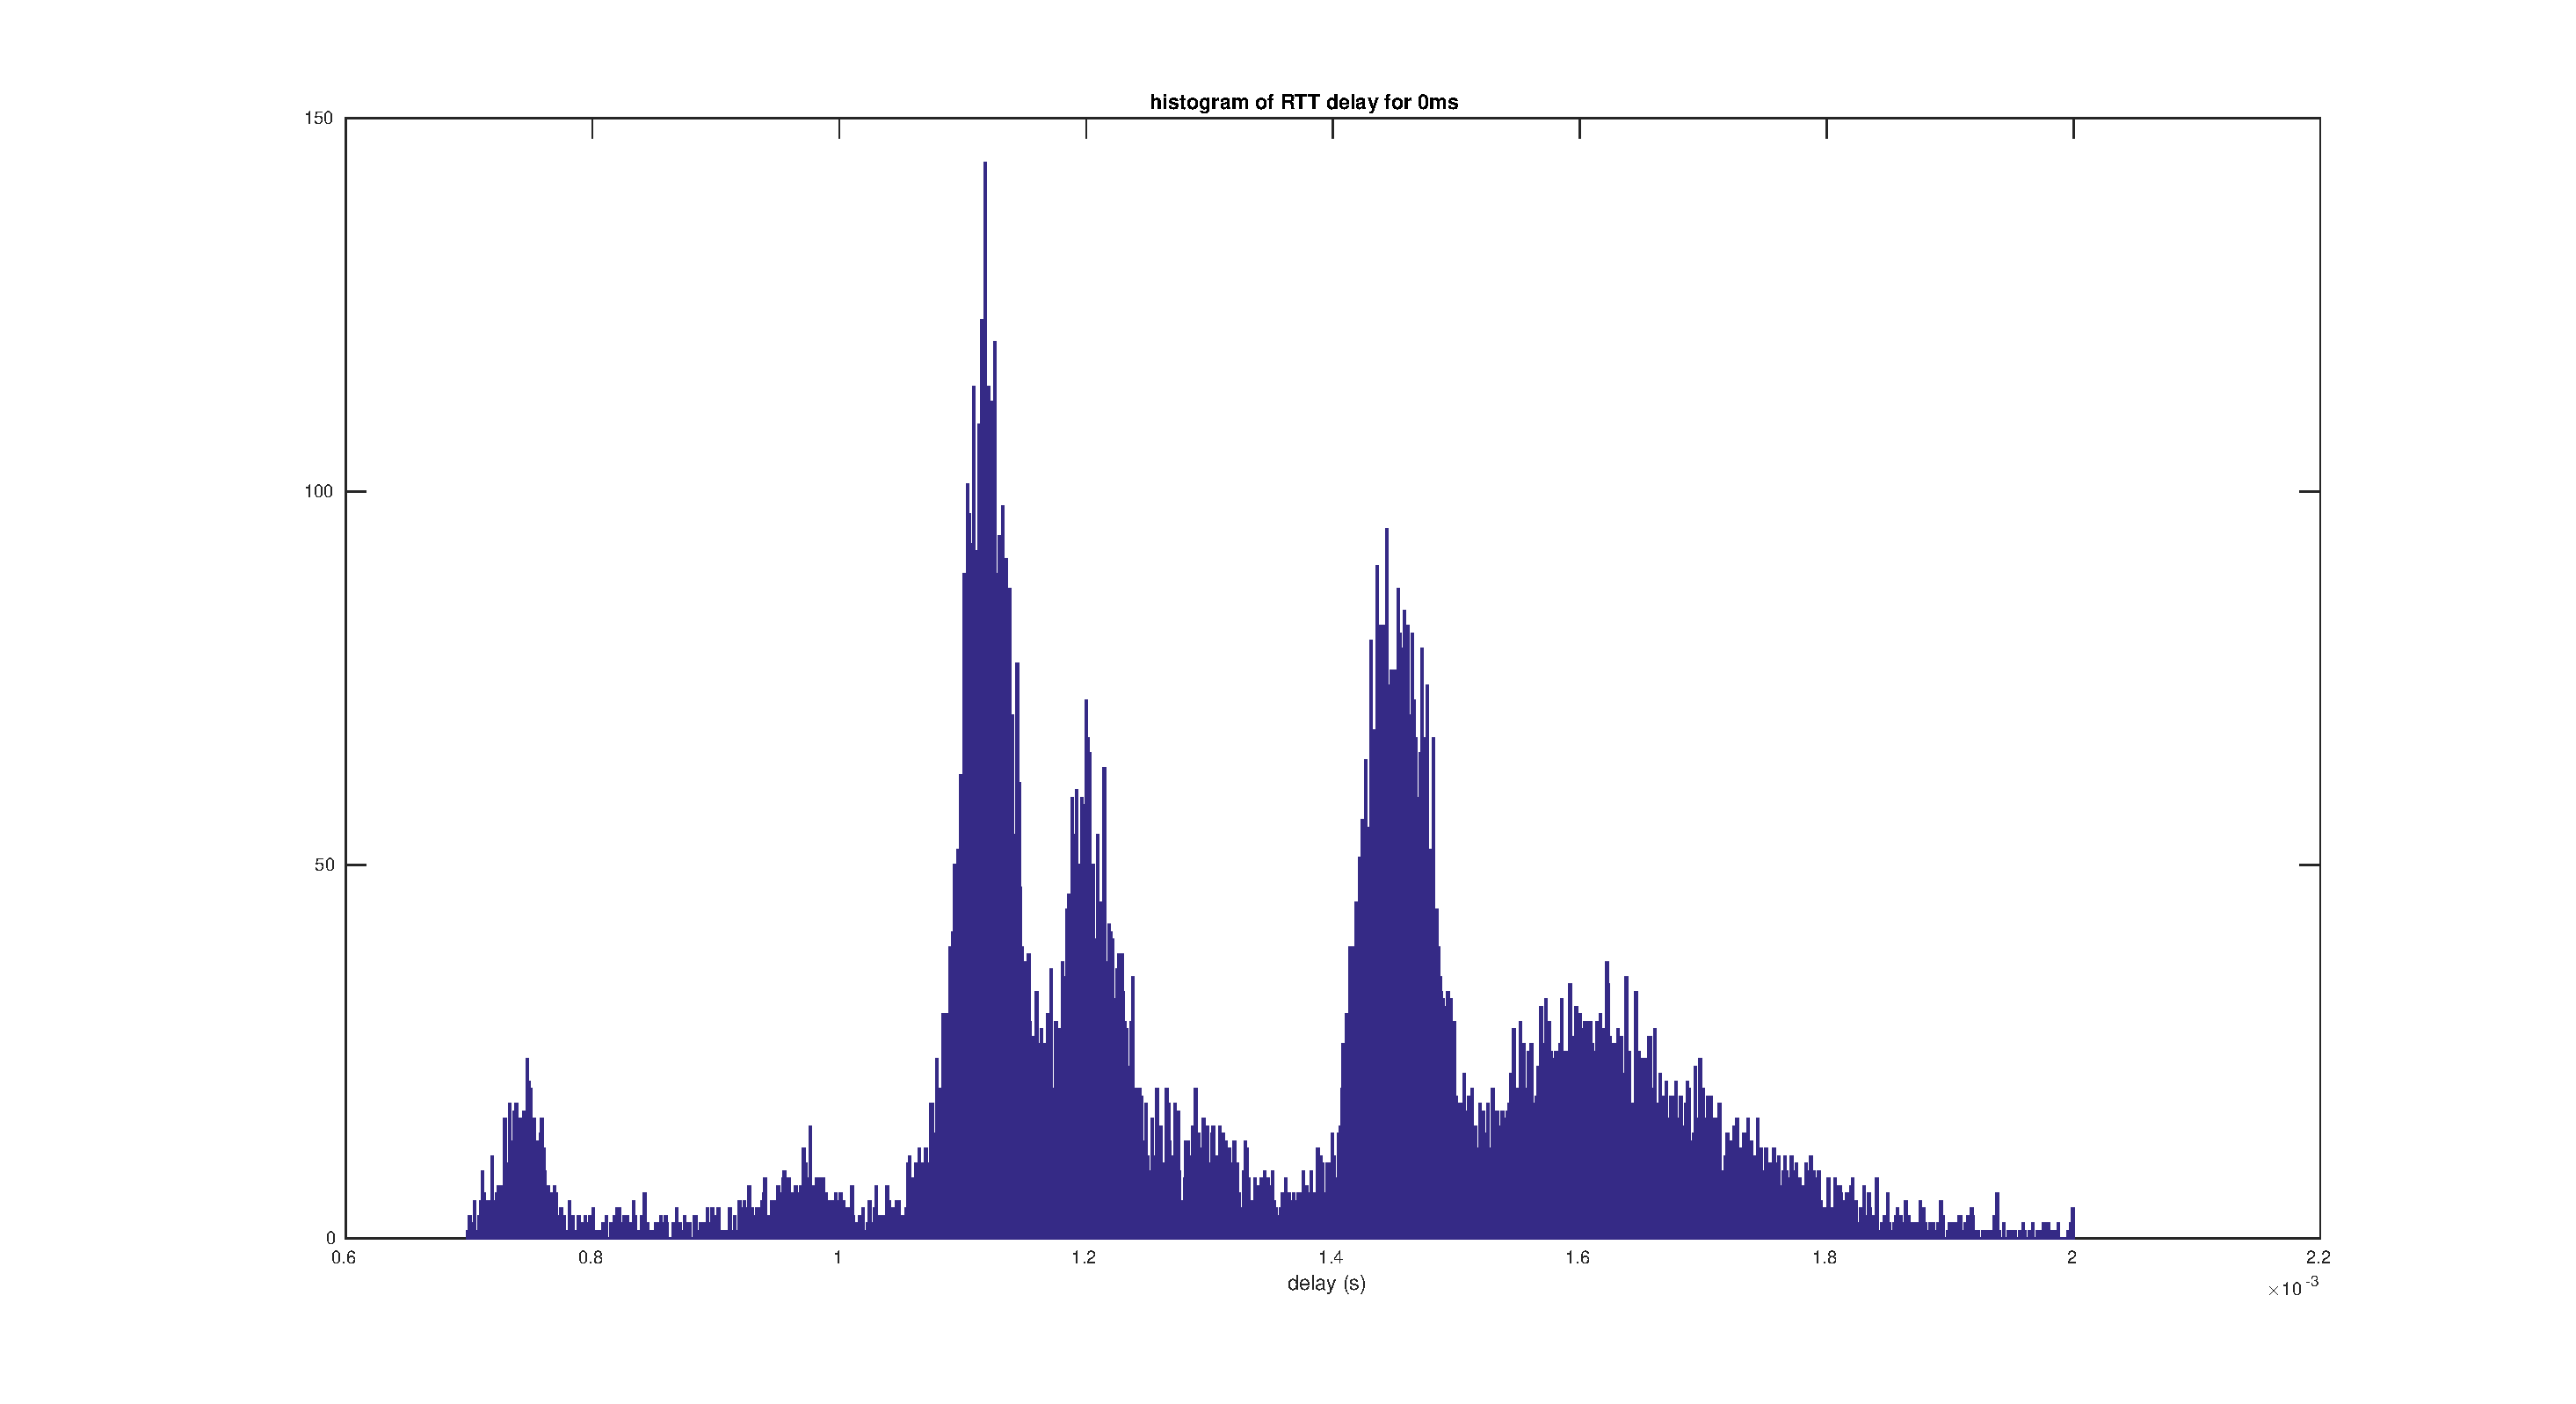
\includegraphics[width=\linewidth]{0ms}
    \caption{0ms}
    \label{fig:0ms}
  \end{subfigure}
\caption{histograms}
\label{fig:histograms}
\end{figure}

When the frequency is increased the jitter increases as well, see Figures \ref{fig:10ms} and \ref{fig:0ms}. This is due to the system becoming more sensitive to disturbances coming from the preemption of other processes.\todo{probably need to justify this}
